\documentclass[oneside,11pt]{amsart}
\usepackage[utf8]{inputenc}%
\usepackage[english]{babel}%
\usepackage{amsmath,amssymb,amsthm,amsfonts}%
\usepackage[unicode]{hyperref}%
\usepackage{mathrsfs,bbm}%
\usepackage{paralist}
\usepackage{color}
\usepackage{longtable}
\usepackage{array}
\newcolumntype{L}[1]{>{\small\raggedright\arraybackslash}m{#1}}
\newcolumntype{T}[1]{>{\footnotesize\raggedright\arraybackslash}m{#1}}
\usepackage{stmaryrd}%
%\usepackage{refcheck}
\usepackage{graphicx}
\usepackage[DIV17]{typearea}
\usepackage{multicol,tikz}
\usepackage{datetime}
\usepackage{cleveref}

\usepackage[shadow]{todonotes}

\usepackage{etoolbox}
\patchcmd{\section}{\scshape}{\Large\itshape\bfseries}{}{}

\usepackage{caption}
\captionsetup{labelformat=empty,labelsep=none}

\hypersetup{
  colorlinks=true,
  linkcolor=blue!50!red,
  urlcolor=green!60!black
}

%%%%%%%%%%%%%%%%%%%%%%%%%%%%%%%%%%%%%%%%%%%%%%%%%%%%%%%%%%%%%%%%%%%%%%%%%%%%%%%%%%%%%%%%
\synctex=1
%%%%%%%%%%%%%%%%%%%%%%%%%%%%%%%%%%%%%%%%%%%%%%%%%%%%%%%%%%%%%%%%%%%%%%%%%%%%%%%%%%%%%%%%
%%%%%%%%%%%%%%%%%%%%%%%%%%%%%%%%%%%%%%%%%%%%%%%%%%%%%%%%%%%%%%%%%%%%%%%%%%%%%%%%%%%%%%%%
\newcommand{\score}[1]{\textit{#1}\addtocounter{totalscore}{#1}}
\newcommand{\razdel}[1]{\smallskip\underline{\textbf{#1:}}\smallskip}

\newcommand{\note}[1]{{\sf{}\color{blue}(#1)}}

\begin{document}

\title[MATH 3100: INTRODUCTION TO PROBABILITY]{MATH 3100: INTRODUCTION TO PROBABILITY}
\author{Leonid Petrov\\Fall 2020\\Sections 002 and 003}
\date{Compiled on \today, \currenttime.\\An up to date syllabus is always on \texttt{GitHub} at \url{https://github.com/lenis2000/Syllabi/blob/master/Syllabus_3100_f20.pdf}. For direct PDF download use \href{https://github.com/lenis2000/Syllabi/raw/master/Syllabus_3100_f20.pdf}{\texttt{this link}}.
	\LaTeX{} source with \textit{changes} to the syllabus is \href{https://github.com/lenis2000/Syllabi/blob/master/Syllabus_3100_f20.tex}{\texttt{here}}
(click ``History'').}
\maketitle

\bigskip

\colorbox{yellow}{\parbox{.7\textwidth}{this syllabus is a stub, and will contain full
details by August 25}}

\section{A mathematical study of randomness}

How random is everything around us, and what chance do we have of understanding it? What to do when you're not certain, and how to do it right? How many falling stars will you see as you walk outside one beautiful night? 

Probability theory is a mathematical study of uncertainty. It is a rigorous foundation of statistics --- and many areas of human knowledge operate in a language of statistics nowadays (yes, and robots use it, too!). The course introduces fundamental concepts, ideas, and techniques of probability theory. It will provide you with the foundational mathematical knowledge needed to address the questions above and will help you develop intuition about randomness.


\begin{figure}[h]
	\begin{tabular}{ccc}
		
\includegraphics[height=.32\textwidth]{img/Bond_percolation_p_51.png}
		&\hspace{10pt}
\includegraphics[height=.32\textwidth]{img/Amas_de_percolation_gray.png}
		&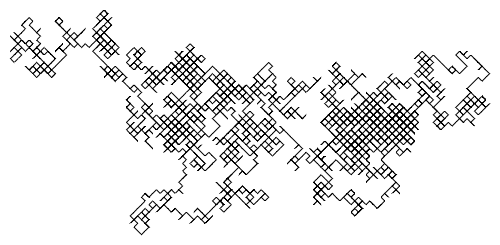
\includegraphics[angle=90,height=.32\textwidth]{img/RW1.png}
	\end{tabular}
	\def\figurename{}
	\caption{Examples of random structures: bond percolation
	\href{https://en.wikipedia.org/wiki/Percolation_theory}{\texttt{close-up}}
	(left),
	at a \href{https://commons.wikimedia.org/wiki/File:Amas_de_percolation.png}{\texttt{larger scale}} (center),
	and
	a 
	\href{https://en.wikipedia.org/wiki/Random_walk\#Lattice_random_walk}{\texttt{random walk}}
	(see also a
	\href{https://upload.wikimedia.org/wikipedia/commons/f/f3/Random_walk_2500_animated.svg}{\texttt{simulation}} 
	of a random walk).
	\tiny{Note:
	this PDF has green clickable links, like in the previous sentence.}
	}
\end{figure}

\subsection*{What you will get from this course}

\begin{enumerate}[\bf{}1.]
	\item Mastery of basic probability concepts:
	\begin{enumerate}[(a)]
		\item What is a probability space and how to translate commonly-sounding problems into this language;
		\item How to count (in an advanced way) to compute probabilities;
		\item What is a random variable, a probability distribution,
		and what are their main quantitative properties;
		\item 
		How commonly encountered probability 
		distributions (binomial, Poisson, exponential, Gaussian) look like and behave,
		what are 
		their properties, and in which situations they typically arise.
	\end{enumerate}

	\item How large random systems behave, and what the 
	bell-shaped curve
	\raisebox{-8pt}{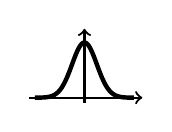
\begin{tikzpicture}
		[scale=.7]
		\draw[ultra thick, domain=-.9:.9] plot[samples=300] ({\x}, {2.7128^(-10*\x*\x)});
		\draw[->, thick] (-1.01,0)--(1.05,0);
		\draw[->, thick] (0,-.1)--(0,1.25);
	\end{tikzpicture}}
	has to do with this.
	\item How to describe and quantify the mutual dependence of random events,
	and how to use such a description 
	to infer properties of ``hidden'' random events.
	\item How to apply probability theory to model real-life processes like queues
	(consisting of people or requests at an internet server).
	\item How to collaborate on solving probability problems in pairs, small groups, and online,
	and present solutions clearly and efficiently.
	% \item How to design probability problems (for example, for the
	% final exam), and evaluate problems presented by others.
	\item In what ways probability theory is connected to science,
	engineering, and other branches of knowledge.
\end{enumerate}

\subsection*{Prerequisite} You should have taken at least one semester of calculus (MATH 1320 level):
the study of random variables often requires single and double integrals
and infinite series.

\subsection*{What this course is and what it is not}

This course in probability \emph{theory} belongs to pure mathematics, with
rigorous definitions, calculations, and proofs. However, the objects which we
study are motivated by real-life applications, and so pure mathematical
arguments often appeal to our common sense understanding of these objects.
There will be opportunities to explore (and discover new) connections of the
theory studied in the course with the real world.

Also, this course does not thoroughly discuss \emph{applications to statistics}
Probability
theory focuses on developing the mathematical side, and statistics applies
these mathematical theories to real data (coming from observations). In this
course we will not discuss how to analyze data coming from observations ---
there are courses in statistics for that.

\section{Necessary information}
\label{sec:necc}

\subsection{Meeting times}{\ }\\

\begin{tabular}{|r|l|l|}
	\hline
	&Section 002&Section 003
	\\
	\hline
	\textbf{Class times}  & TuTh 11:00AM - 12:15PM &TuTh 12:30PM - 1:45PM
                       \\ \hline
											 \textbf{Midterm 1}   & TBA & TBA                       
                       \\ \hline
											 \textbf{Midterm 2}   & TBA & TBA
											 \\ \hline
											 \textbf{Final exam}   &  
										 Thursday, \textbf{December 10, 2020}	
											 & 
											 Wednesday, \textbf{December 02, 2020}	
											 \\ & 9:00AM-12:00PM &  2:00PM-5:00PM
                       \\ \hline
\end{tabular}

\bigskip

	\textbf{Instructor:} Leonid Petrov

	\textbf{Course communication:} We use \texttt{Piazza}, see \Cref{comm}

	\textbf{Office hours:} 
	TBA, 
	and by appointment.
	
	You can automatically schedule an office hours appointment 
	at \href{https://lpetrov.cc/teaching/}{this page} (please don't make an appointment for 
	regular office hours).
	You can make as many appointments as you need throughout the semester. Each appointment
	must be made at least 3 hours prior to the time of the appointment.
	
	\textbf{Course delivery:} TBA


\subsection{About the instructor}
I am an Associate Professor in the Department of Mathematics at UVA, and I've
been here since 2014. My research area is probability theory (very appropriate
for this course!). More precisely, I am using exact formulas to study large
random systems. I also like computer simulations of random systems like 
\href{https://d3m0khvr0ybm92.cloudfront.net/img/blog/heart/UVA_colors_small.png}{\texttt{this one}}.
I'm happy to tell you more if you're
interested.

\subsection{Textbook}
Anderson, Sepp\"al\"ainen, Valk\'o, \emph{Introduction to Probability}, 1st Edition.

ISBN-13: 978-1108415859; 
ISBN-10: 9781108415859.

See also \Cref{success} below for discussion 
of how we'll use the textbook,
and for other helpful resources.

\section{Assessing your learning}

Learning mathematics means \emph{doing} mathematics: during class meetings, on your own, and in groups.
In this course, doing mathematics mainly amounts to solving problems.
The following aspects are assessed in this course:

TBA

\subsection*{Letter grades}

The scale by which course percent grades are turned into course letter grades
will most likely be the following:
\begin{equation*}
	\begin{tabular}{l|l|l|l|l|l|l|l|l|l|l|l|l|}
		Grade      & $ A+	$ & $A	$ & $A-	$ & $B+	$ & $B	$ & $B-	$ & $C+	$ & $C	$ & $C-	$ & $D+	$ & $D	$ & $D-$ \\
		\hline
		Minimum \% & 100     & 93   & 89    & 86    & 82    & 79    & 76    & 72    & 69    & 66    & 62    & 59
	\end{tabular}
\end{equation*}
I reserve the right to slightly change this grade scale after the
final exam.
This may be needed
to better incorporate into the letter grade
possible fluctuations in the difficulty level of 
midterms and the final.

\section{Communication}
\label{comm}

\subsection{Email}

My email address is \href{mailto:petrov@virginia.edu}{petrov@virginia.edu}.

\subsection{Piazza}

TBA

\subsection{Collab}

TBA.

If you have anonymous comments on anything related to the course, you can make
them via Collab.

\section{How to succeed in the course}
\label{success}

\subsection{General things}

The best way to learn in the course is to 
watch all recorded lectures and take notes to retain the material in memory; 
come to all discussion meetings;
and do all the homework problems on your own or in collaboration.
This will prepare you well for tests.

\subsection{Main textbook}

The textbook \emph{Introduction to Probability} by Anderson, Sepp\"al\"ainen, and Valk\'o 
is 
an excellent resource 
to gain understanding of the course material. Some notes about it:

\begin{enumerate}[$\bullet$]
	\item I strongly encourage you to read the textbook in parallel with watching the lectures. 
		It includes many examples and
		extra exercises which augment the concepts discussed in class.
	\item The textbook contains much more material than will be covered in classes, so it
		makes sense to watch lectures and come to discussions to note which parts are omitted
		(and so won't be in tests).
\end{enumerate}

\subsection{Additional textbooks}

\begin{enumerate}
	\item 
		\emph{``Probability'' by Jim Pitman} is a reasonable alternative textbook.
	\item 
		\emph{Free textbook} 
		\emph{``Introduction to Probability'' by Grinstead and Snell}.
			Download: \url{https://math.dartmouth.edu/~prob/prob/prob.pdf};
			Accompanying web page: \url{https://www.dartmouth.edu/~chance/teaching_aids/books_articles/probability_book/book.html}.
\end{enumerate}

These textbooks contain additional problems and material. They may be helpful if you want
a deeper understanding of some concepts, or if you want to read exposition of the familial material
in a different style, which might be very helpful for better learning.

(It absolutely not required that you buy or read these books.)

\subsection{Extra reading}

The popular book
\emph{``How Not to Be Wrong: The Power of Mathematical Thinking'' by Jordan Ellenberg}
discusses how math touches every aspect of real life, and has 
numerous examples related to probability and statistics. 
I can recommend this nice book as a parallel reading. Some
examples I learned from this book might be mentioned in class.
(It absolutely not required that you buy or read this book.)

\subsection{Other resources}

There is a number of online resources which may help you while doing the homework:
Khan Academy, Wikipedia, and many other 
places contain lots of basic material on probability theory. Google Search
in general
is also a valuable resource.

\subsection{Office hours}

I am available during office hours to answer questions on the content of the 
course, clarify various points, and I can also help you with homework assignments. 
Besides regular office hours, you can automatically schedule appointments, see 
\Cref{sec:necc}.

\subsection{Math Collaborative Learning Center}

The Math Department 
Collaborative Learning Center
is available for helping students in this course: 
see \url{https://math.virginia.edu/undergraduate/MCLC/}
for more information and schedule. 

\subsection{Piazza}

TBA

\subsection{Collaboration on homework assignments}
\label{collaboration}

Group work on homework problems is allowed and strongly encouraged.
Discussions are in general very
helpful and inspiring. Class meetings will also contain ample time
for group work on homework problems.
Nevertheless, before talking to others, get well started
on the problems, and contribute your fair share to the process. 

When completing the written homework assignments, everyone must write up his or her own
solutions in their own words, and cite any reference 
(other than the textbook and
class notes) that you use. Quotations and citations are part of the Honor Code for both UVa
and the whole academic community. 

It is very important that you truly understand the homework solutions you hand
in, otherwise you may be unpleasantly surprised by your test results.

\section{Approximate course schedule}

\noindent Add/drop information: \url{https://www2.virginia.edu/registrar/reginst1208.html}
\bigskip

% \begin{quote}
%   The course has 3 ``pillars'': central limit theorem for Gaussian approximation,
%   Poisson processes, and conditional expectations.
%   Plus there are several technical things to learn: random variables, expectations as integrals,
%   joint distributions, etc.
% \end{quote}
%
% \bigskip

\begin{enumerate}[\bf{}{[}week 1{]}]
	\item 8/25, 8/27.
	\item 

\end{enumerate}

\section{Policies}

\subsection{Late/make up work} Each assignment will have due date and time.
Late assignments are not accepted. There will also be no make up for the midterm test.
However, if you have special needs, emergency, or unavoidable conflicts, please
let me know as soon as possible, so we can arrange a workaround.

\subsection{Special needs}

All students with special needs requiring accommodations should present the
appropriate paperwork from the Student Disability Access Center (SDAC). It is
the student's responsibility to present this paperwork in a timely fashion and
follow up with the instructor about the accommodations being offered.
Accommodations for test-taking (e.g., extended time) should be arranged at
least 5 business days before an exam.

\subsection{Honor Code} The University of Virginia Honor Code applies to this
class and is taken seriously (in particular, 
see \Cref{collaboration} on homework collaboration).
Any honor code violations will be referred to the
Honor Committee.











\end{document}
